\documentclass[a4paper]{article}
\usepackage[utf8]{inputenc}
\usepackage[russian,english]{babel}
\usepackage[T2A]{fontenc}
\usepackage[left=10mm, top=20mm, right=18mm, bottom=15mm, footskip=10mm]{geometry}
\usepackage{indentfirst}
\usepackage{amsmath,amssymb}
\usepackage[italicdiff]{physics}
\usepackage{graphicx}
\usepackage{caption}
\usepackage{float}
\renewcommand{\thefootnote}{\fnsymbol{footnote}}
\usepackage{tablefootnote}
\usepackage{footmisc}
\usepackage[parfill]{parskip}
\usepackage[utf8]{inputenc}\newcommand{\approxtext}[1]{\ensuremath{\stackrel{\text{#1}}{\approx}}}
\graphicspath{{images/}}
\DeclareGraphicsExtensions{.pdf,.png,.jpg}
\usepackage{wrapfig}
\captionsetup{labelformat=empty}
\usepackage{caption}
\captionsetup[figure]{name=Рисунок}
\captionsetup[table]{name=Таблица}
  
\title{\textbf{Отчет о выполненой лабораторной работе 2.1.6}}
\date{}
\author{Котляров Михаил, Б01-402}

\begin{document}

\maketitle
	
	\section{Введение}
	
	\textbf{Цель работы:} : 1) определить изменения температуры углекислого газа при протекании через малопроницаемую перегородку при разных начальных значениях температуры, вычислить коэффициент Джоуля-Томсона; 2) вычислить по результатам опытов коэффициенты $a$ и $b$ модели Вандер-Ваальса, а также температуру инверсии $T_{\text{инв}}$.\\

	\textbf{Оборудование:} трубка с пористой перегородкой; труба Дьюара; термостат
жидкостной; термопара; вольтметр универсальный цифрововй; баллон с углекислым газом; манометр.
	
	\section{Теоретические сведения}
\textit{Эффектом Джоуля–Томсона} называется изменение температуры газа, медленно
просачивающегося из области высокого в область низкого давления в условиях тепловой изоляции. В разреженных газах, которые приближаются по своим свойствам
к идеальному, при таком течении температура газа не меняется. Таким образом, в
эффекте Джоуля–Томсона проявляется отличие исследуемого газа от идеального.\\
Получим теоретическое выражения для расчёта величины эффекта Джоуля–Томсона.
Так как через боковые стенки не происходит ни обмена теплом, ни передачи механической энергии, то:
\begin{equation*}
	A_1-A_2 = P_1V_1-P_2V_2 = (U_2 + \mu v_2^2/2) - (U_1+\mu v_1^2/2),
\end{equation*}
\begin{equation*}
	H_1-H_2 = \frac{\mu}{2} (v_2^2/2 - v_1^2/2).
\end{equation*}
\begin{figure}[h!]
        \centering
        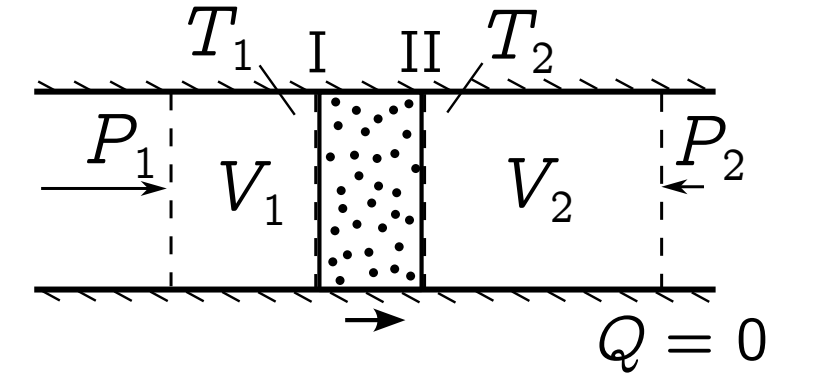
\includegraphics[scale=0.5]{Pictures/Scheme.png}
        \caption{
        Рис. 1. Принципиальная схема эффекта Джоуля–Томсона
        }
 \end{figure} 



Правая часть оказывается принебрежимо малой. Тогда приходим к выводу, что эффект Джоуля-Томсона — это процесс, в котором сохраняется энтальпия:
\begin{equation*}
	H_1 \approx H_2 .
\end{equation*}
Энтальпия — функция состояния, зависящая, в общем случае, как от температуры T, так и от давления P. Поэтому в результате просачивания газа под действием
перепада давления, равного по модулю $|\Delta P| = P_1 - P_2$, возникнет изменение его температуры $\Delta T = T_2 - T_1$. Коэффициентом Джоуля–Томсона называют отношение
\begin{equation*}
	\mu_{\text{Д-Т}} = \frac{\Delta T} {\Delta P}.
\end{equation*}
Рассмотрим простейшую модель реального газа: газ Ван-дер-Ваальса. Термическое и калорическое уравнения состояния для него, как известно, имеют следующий вид:
\begin{equation*}
	(P + \frac{a}{V^2})(V - b) = RT,
\end{equation*}

\begin{equation*}
	U = C_VT - \frac{a}{V}.
\end{equation*}
Энтальпия газа Ван-дер-Ваальса:
\begin{equation*}
	H = U + PV = C_VT + RT\frac{V}{V - b} - \frac{2a}{V}.
\end{equation*}
Для упрощения можно воспользоваться следующим обстоятельством: газ в опыте
является достаточно разреженным (его давление не превышает 5 атм) и довольно
близок к идеальному. Поэтому его отличия от идеального следует учитывать только
в эффекте Джоуля–Томсона, но не при вычислении объёма V по известным T и P. То
есть, будем считать $V \approx \frac{RT}{P}$, $\frac{V}{V-b} \approx 1 + \frac{b}{V}$, $C_V + R \approx C_P$. В результате получим:
\begin{equation*}
	H \approx C_PT + P(b - \frac{2a}{V}),
\end{equation*}
\begin{equation*}
	\mu_{\text{Д-Т}} = \frac{\Delta T} {\Delta P} \approx \frac{\frac{2a}{RT} - b} {C_P}.
	\eqno(1)
\end{equation*}

\section{Экспериментальная установка}
Схема установки для исследования эффекта Джоуля–Томсона в углекислом газе
представлена на рис. 2. Основным элементом установки является трубка 1 с пористой
перегородкой 2, через которую пропускается двуокись углерода $CO_2$. Углекислый газ под повышенным давлением поступает в трубку через змеевик 5
из балластного баллона 6. Медный змеевик омывается водой и нагревает медленно
протекающий через него газ до температуры воды в термостате. Температура воды
измеряется встроенным в термостат термометром. Давление газа в трубке измеряется манометром М и регулируется вентилем В . Манометр М измеряет разность между давлением внутри трубки и наружным (атмосферным) давлением. Разность температур газа до и после перегородки измеряется термопарой медь–константан.
\begin{figure}[h!]
        \centering
        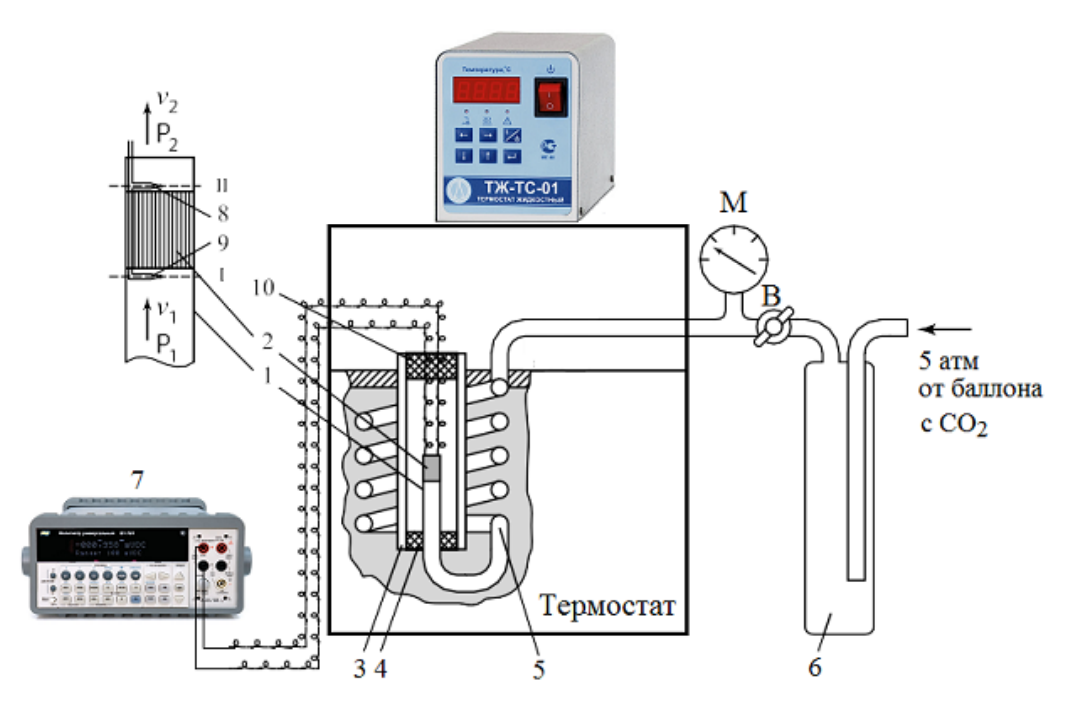
\includegraphics[scale=0.5]{Pictures/ustanovka.png}
        \caption{
        Рис. 2. Экспериментальная установка
        }
 \end{figure} 


\section{Приборы и данные}
\begin{itemize}
    \item Цифровые мультиметры Вольтметр универсальный B7-78/1, погрешность измерения погрешность измерения постоянного напряжения 0,0035\% + 0,0005\% диапазона. 
    \item Термостат жидкостный ТЖ-ТС-01, предел допускаемой погрешности установления заданной температуры не более $0,02 ^\circ C$, погрешность поддержания температуры не более $0,01 ^\circ C$.
    \item Манометр WIKA EN 837-1, класс точности 1,0.
\end{itemize}
\section{Выполнение}
\begin{enumerate}

\item Начальные показания приборов
\begin{equation*}
	t_0 = 13,9 ^\circ C;		\varepsilon_0 = -0,002 \text{мВ},
\end{equation*}
где $t_0$ - начальная температура термостата с водой, $\varepsilon_0$ - показания вольтметра\\
\textbf{ВАЖНО!} Для уточнения, далее все значения напряжений на термопаре $\varepsilon$, указаны по модулю, но на мультиметре все они были отрицательными.

\item В каждой серии экспериментов для каждой температуры воды в термостате будем устанавливать давление и, когда показания вольтметра перестанут меняться, будем фиксировать напряжение на термопаре. Погрешность напряжения складывается из систематической погрешности и погрешности колебания величины. Поскольку $\sigma_\varepsilon ^{\text{сист}} \ll \sigma_\varepsilon ^{\text{колеб}} $, то
\begin{equation*}
	\sigma_\varepsilon = \sqrt{{\sigma_\varepsilon ^{\text{сист}}} ^ 2 + {\sigma_\varepsilon ^{\text{колеб}}} ^ 2} \approx \sigma_\varepsilon ^{\text{колеб}} = 0,001 \text{мВ}.
\end{equation*}
Разница температур термопары определяется по формуле $\Delta T = \frac{\Delta \varepsilon} {\frac{d\varepsilon}{d T}} $. Значения чувствительности медно-константановой термопары взяты из описания к работе.
Далее приведены экспериментальные значения.
\begin{table}[h!]
    \centering
    \begin{tabular}{|c|c|c|c|c|c|}
        \hline
        $T, ^\circ C$ & $P, \text{бар}$ & $\varepsilon, \text{мВ}$ & $\Delta T, ^\circ C$ & $\sigma_{\Delta T}, ^\circ C$ & $\varepsilon_{\Delta T}, \%$ \\
        \hline
        $15.22 \pm 0.02$ & $4.10 \pm 0.06$ & $0.140 \pm 0.001$ & 3.518 & 0.025 & 0.71 \\ \hline
        $15.33 \pm 0.02$ & $3.50 \pm 0.06$ & $0.111 \pm 0.001$ & 2.789 & 0.025 & 0.90 \\ \hline
        $15.45 \pm 0.02$ & $3.00 \pm 0.06$ & $0.083 \pm 0.001$ & 2.085 & 0.025 & 1.20 \\ \hline
        $15.60 \pm 0.02$ & $2.50 \pm 0.06$ & $0.065 \pm 0.001$ & 1.633 & 0.025 & 1.54 \\ \hline
    \end{tabular}
    \caption{Таблица 1. Диапазон температуры 15,22\textdiv15,60 $^\circ C$}
\end{table}

\begin{table}[h!]
    \centering
    \begin{tabular}{|c|c|c|c|c|c|}
        \hline
        $T, ^\circ C$ & $P, \text{бар}$ & $\varepsilon, \text{мВ}$ & $\Delta T, ^\circ C$ & $\sigma_{\Delta T}, ^\circ C$ & $\varepsilon_{\Delta T}, \%$ \\
        \hline
        $33.07 \pm 0.02$ & $4.05 \pm 0.06$ & $0.116 \pm 0.001$ & 2.795 & 0.024 & 0.86 \\ \hline
        $33.04 \pm 0.02$ & $3.50 \pm 0.06$ & $0.090 \pm 0.001$ & 2.169 & 0.024 & 1.11 \\ \hline
        $33.02 \pm 0.02$ & $3.00 \pm 0.06$ & $0.070 \pm 0.001$ & 1.687 & 0.024 & 1.43 \\ \hline
        $33.00 \pm 0.02$ & $2.40 \pm 0.06$ & $0.051 \pm 0.001$ & 1.229 & 0.024 & 1.96 \\ \hline
        $33.00 \pm 0.02$ & $1.90 \pm 0.06$ & $0.035 \pm 0.001$ & 0.843 & 0.024 & 2.86 \\
        \hline
    \end{tabular}
    \caption{Таблица 2. Диапазон температуры 33,00\textdiv33,07 $^\circ C$}
\end{table}

\begin{table}[h!]
    \centering
    \begin{tabular}{|c|c|c|c|c|c|}
        \hline
        $T, ^\circ C$ & $P, \text{бар}$ & $\varepsilon, \text{мВ}$ & $\Delta T, ^\circ C$ & $\sigma_{\Delta T}, ^\circ C$ & $\varepsilon_{\Delta T}, \%$ \\
        \hline
        $45.04 \pm 0.02$ & $4.10 \pm 0.06$ & $0.107 \pm 0.001$ & 2.524 & 0.024 & 0.93 \\ \hline
        $45.02 \pm 0.02$ & $3.50 \pm 0.06$ & $0.082 \pm 0.001$ & 1.934 & 0.024 & 1.22 \\ \hline
        $45.00 \pm 0.02$ & $3.00 \pm 0.06$ & $0.066 \pm 0.001$ & 1.557 & 0.024 & 1.52 \\ \hline
        $45.00 \pm 0.02$ & $2.60 \pm 0.06$ & $0.050 \pm 0.001$ & 1.179 & 0.024 & 2.00 \\ \hline
        $45.00 \pm 0.02$ & $1.80 \pm 0.06$ & $0.028 \pm 0.001$ & 0.660 & 0.024 & 3.57 \\
        \hline
    \end{tabular}
    \caption{Таблица 3. Диапазон температуры 45,00\textdiv45,04 $^\circ C$}
\end{table}

\begin{table}[h!]
    \centering
    \begin{tabular}{|c|c|c|c|c|c|}
        \hline
        $T, ^\circ C$ & $P, \text{бар}$ & $\varepsilon, \text{мВ}$ & $\Delta T, ^\circ C$ & $\sigma_{\Delta T}, ^\circ C$ & $\varepsilon_{\Delta T}, \%$ \\
        \hline
        $56.91 \pm 0.02$ & $4.10 \pm 0.06$ & $0.102 \pm 0.001$ & 2.361 & 0.023 & 0.98 \\ \hline
        $56.92 \pm 0.02$ & $3.40 \pm 0.06$ & $0.076 \pm 0.001$ & 1.759 & 0.023 & 1.32 \\ \hline
        $56.93 \pm 0.02$ & $3.00 \pm 0.06$ & $0.061 \pm 0.001$ & 1.412 & 0.023 & 1.64 \\ \hline
        $56.94 \pm 0.02$ & $2.50 \pm 0.06$ & $0.046 \pm 0.001$ & 1.065 & 0.023 & 2.17 \\ \hline
        $56.96 \pm 0.02$ & $2.00 \pm 0.06$ & $0.030 \pm 0.001$ & 0.694 & 0.023 & 3.33 \\
        \hline
    \end{tabular}
    \caption{Таблица 4. Диапазон температуры 56,91\textdiv56,96 $^\circ C$}
\end{table}
\clearpage
\item По этим данным построим по МНК графики зависимости разности температур от перепада давления $\Delta T(\Delta P) $ для разных температур.
\begin{figure}[h!]
\centering{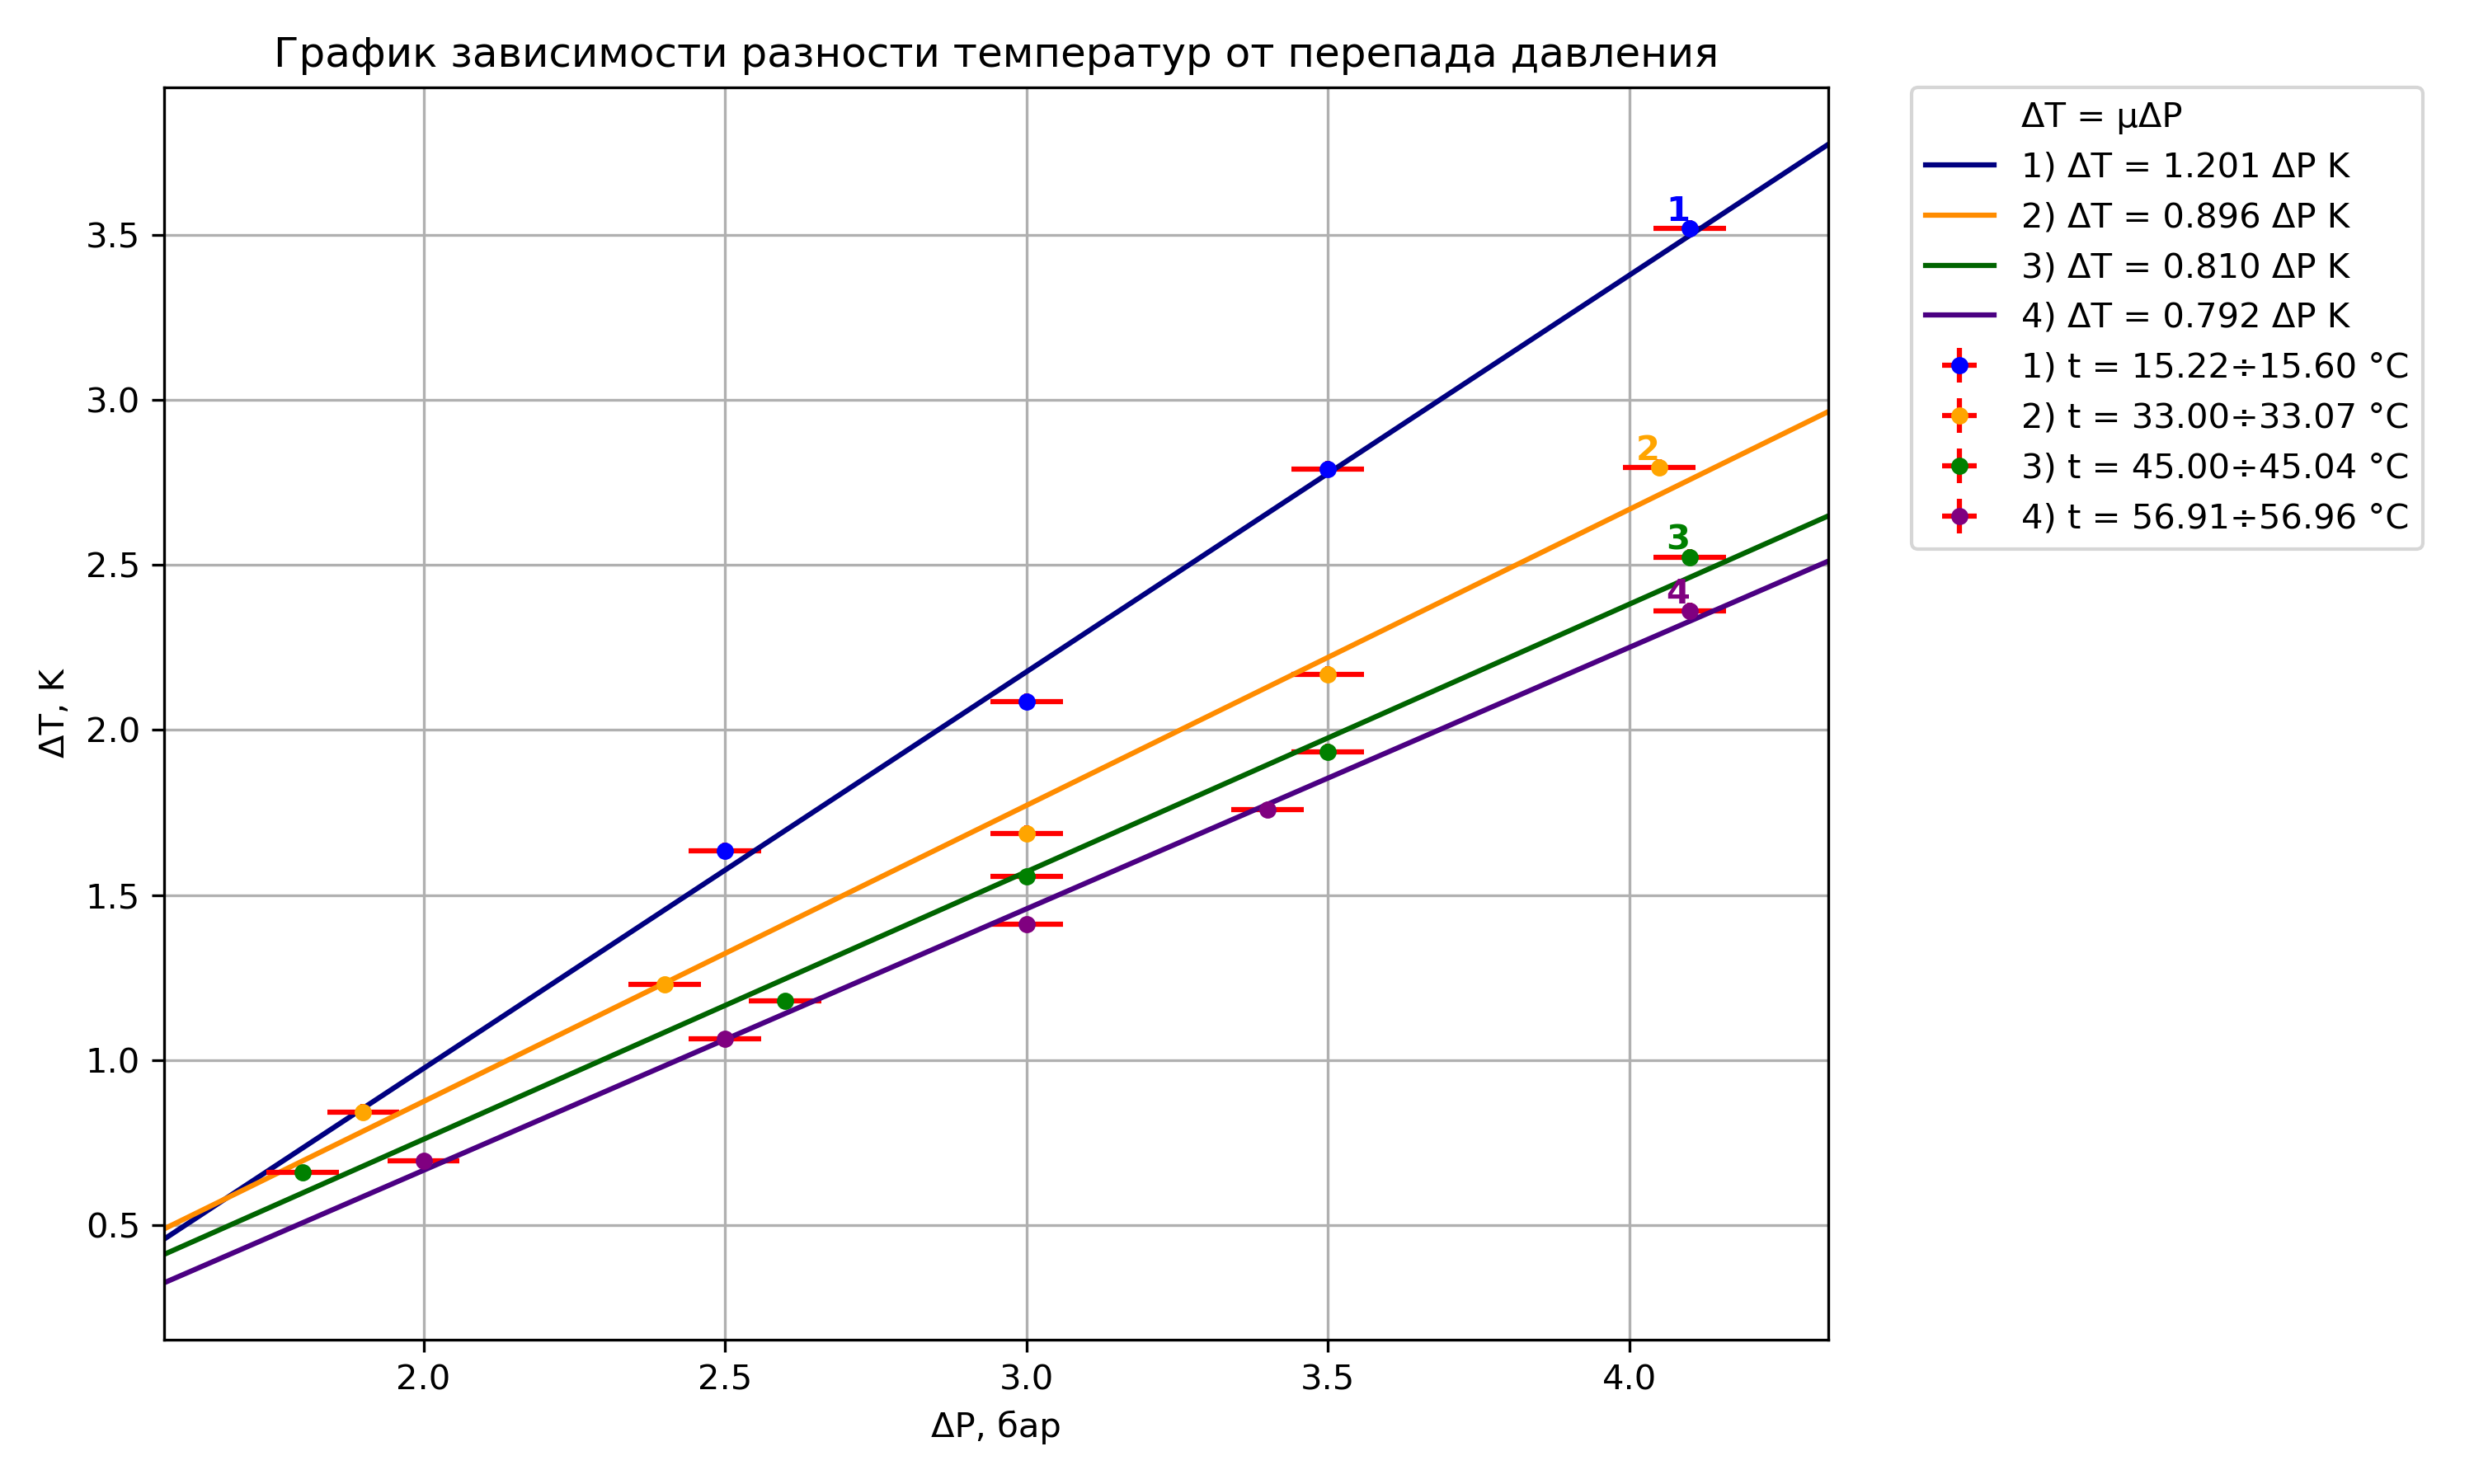
\includegraphics[width=1\textwidth]{Graphics/graph1.png}}
\caption[]{\label{} График №1 Зависимость разности температур от перепада давления $\Delta T(\Delta P)$}
\end{figure}

По наклону прямых получим значения коэффициентов Джоуля-Томсона для разных температур воды в термостате. 
\begin{table}[h!]
    \centering
    \begin{tabular}{|c|c|c|c|}
        \hline
        № & $\mu_{\text{Д-Т}}, \frac{\text{К}}{\text{бар}}$ & $\sigma_{\mu_{\text{Д-Т}}}, \frac{\text{К}}{\text{бар}}$ & $\varepsilon, \%$ \\
        \hline
        1 & $1.201$ & $0.046$ & $3.87$ \\
        \hline
        2 & $0.896$ & $0.037$ & $4.12$ \\
        \hline
        3 & $0.810$ & $0.030$ & $3.75$ \\
        \hline
	  4 & 0,792	&0,018&	2,235 \\
	  \hline
    \end{tabular}
    \caption{Таблица 5. Коэффициенты Джоуля-Томсона для серий измерений 1-4}
\end{table}
\renewcommand{\thefootnote}{*}
\item По данным таблицы 5 постром по МНК график зависимости коэффициента Джоуля-Томсона от обратной температуры $\mu_{\text{Д-Т}}(\frac{1}{T})$. Температуру будем брать среднюю из значений для каждого диапазона. Также построим такую зависимость для табличных значений\footnotemark{}  коэффициентов Джоуля-Томсона.

\footnotetext{в данной работе в местах, где не указано, табличные значения были взяты из книги Лабораторный практикум по общей физике Том I Термодинамика и молекулярная физика}
\renewcommand{\thefootnote}{\arabic{footnote}}
\clearpage
\begin{figure}[h!]
\centering{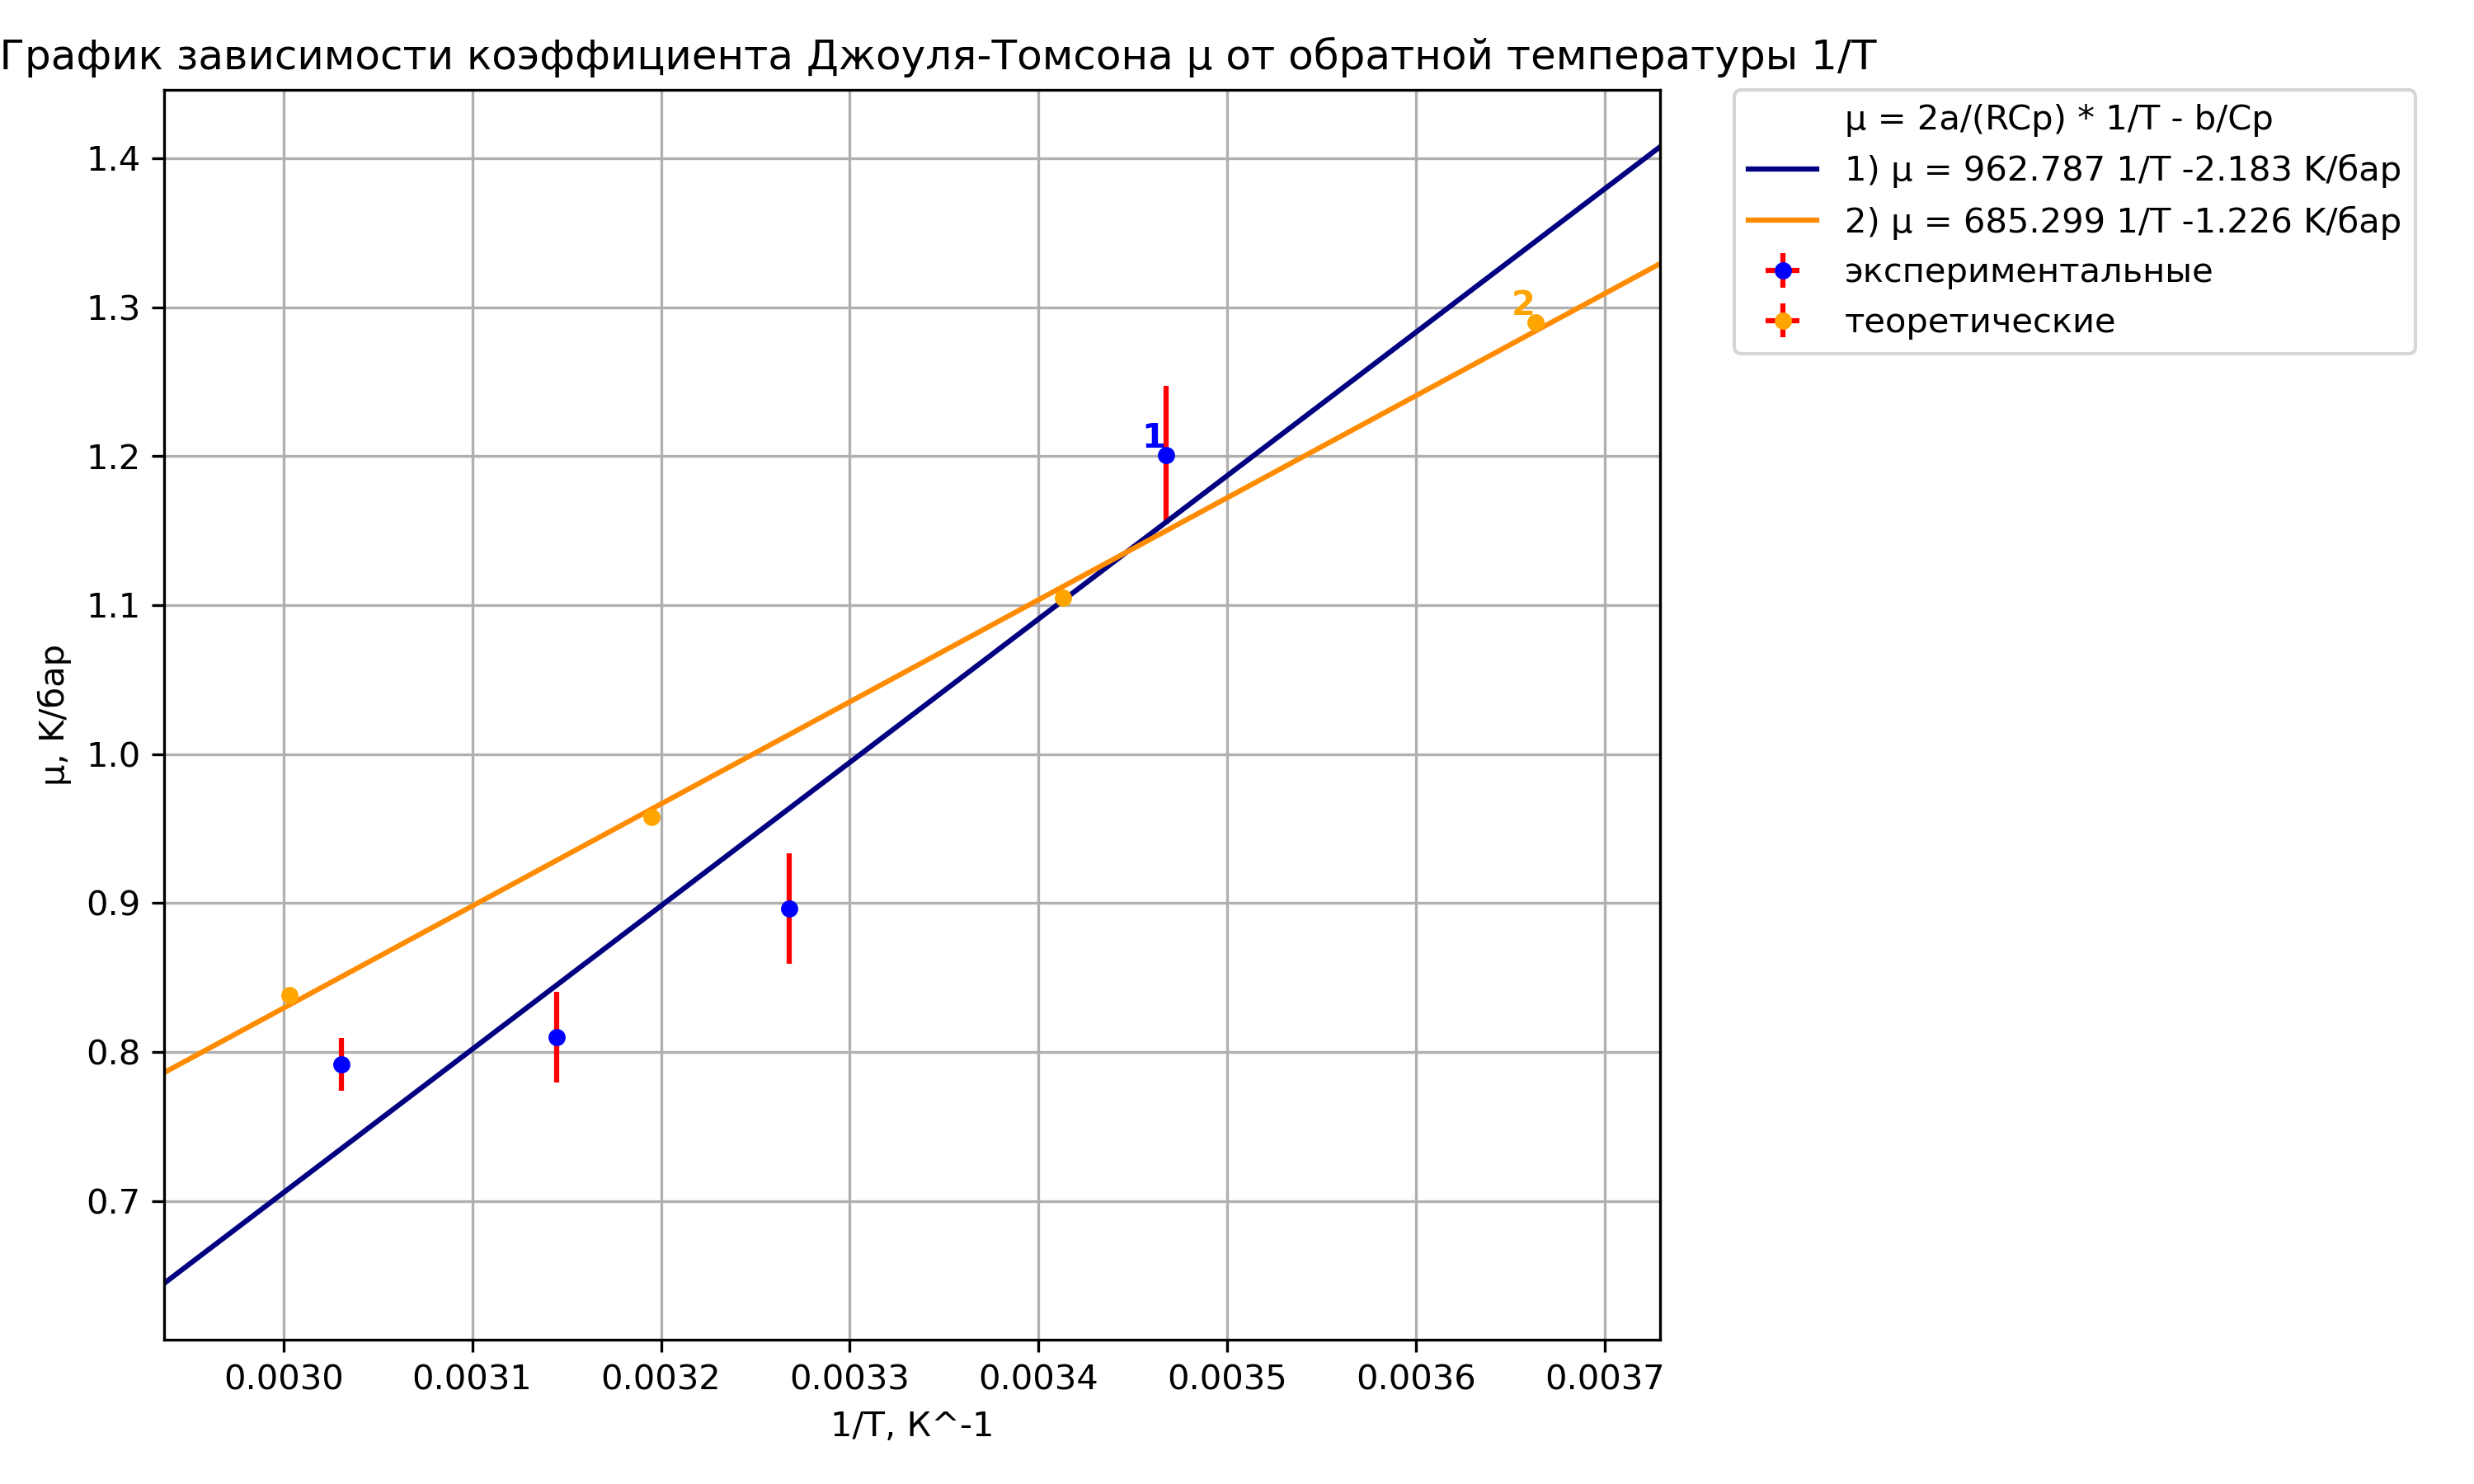
\includegraphics[width=1\textwidth]{Graphics/graph2.png}}
\caption[]{\label{} График 2. Зависимости коэффициента Джоуля-Томсона от обратной температуры $\mu_{\text{Д-Т}}(\frac{1}{T})$}
\end{figure}

По наклонам прямых $k$ и пересечению с осью ординат $\mu_0 = -\frac{b}{C_p}$ определим коэффициенты $a$ и $b$ в уравнении состояния газа Ван-дер-Ваальса. Примем $R = 8,31 \frac{\text{Дж}}{\text{моль}\cdot K}$ и значение $C_p = 37,1 \frac{\text{Дж}}{\text{моль}\cdot K}$ возьмем из таблицы.
\begin{equation*}
	k^{\text{эксп}} = 963 \pm 161 \frac{K^2}{\text{бар}} \Rightarrow a^{\text{эксп}} = \frac{k^{\text{эксп}} R C_p}{2} = 1,484 \frac{H\cdot\text{ м} ^4}{\text{моль} ^2},
\end{equation*}
\begin{equation*}
	\sigma_{a^{\text{эксп}}} = a^{\text{эксп}} \frac{\sigma_{k^{\text{эксп}}}}{k^{\text{эксп}}} = 0,249 \frac{H\cdot\text{ м} ^4}{\text{моль} ^2},
\end{equation*}
\begin{equation*}
	a^{\text{эксп}} = 1,484 \pm 0,249 \frac{H\cdot\text{ м} ^4}{\text{моль} ^2}(\varepsilon = 16,75\%),
\end{equation*}

\begin{equation*}
	\mu_0^{\text{эксп}} = -2,183 \pm 0,026 \frac{K}{\text{бар}} \Rightarrow b^{\text{эксп}} = \mu_0^{\text{эксп}} C_p = 8,10 \cdot 10^{-4} \frac{\text{м} ^3}{\text{моль}},
\end{equation*}
\begin{equation*}
	\sigma_{b^{\text{эксп}}} = b^{\text{эксп}} \frac{\sigma_{\mu_0^{\text{эксп}}}}{\mu_0^{\text{эксп}}} = 0,18 \cdot 10^{-4} \frac{\text{м} ^3}{\text{моль}},
\end{equation*}
\begin{equation*}
	b^{\text{эксп}} = (8,10 \pm 0,18) \cdot 10^{-4} \frac{\text{м} ^3}{\text{моль}}  (\varepsilon = 2,18\%),
\end{equation*}

\begin{equation*}
	k^{\text{табл}} = 685 \pm 54 \frac{K^2}{\text{бар}} \Rightarrow a^{\text{табл}} = \frac{k^{\text{табл}} R C_p}{2} = 1,043 \frac{H\cdot\text{ м} ^4}{\text{моль} ^2},
\end{equation*}
\begin{equation*}
	\sigma_{a^{\text{табл}}} = a^{\text{табл}} \frac{\sigma_{k^{\text{табл}}}}{k^{\text{табл}}} = 0,082 \frac{H\cdot\text{ м} ^4}{\text{моль} ^2},
\end{equation*}
\begin{equation*}
	a^{\text{табл}} = 1,043 \pm 0,082 \frac{H\cdot\text{ м} ^4}{\text{моль} ^2}(\varepsilon = 7,84\%),
\end{equation*}

\begin{equation*}
	\mu_0^{\text{табл}} = -1,226\pm 0,013 \frac{K}{\text{бар}} \Rightarrow b^{\text{табл}} = \mu_0^{\text{табл}} C_p = 4,490 \cdot 10^{-4} \frac{\text{м} ^3}{\text{моль}},
\end{equation*}
\begin{equation*}
	\sigma_{b^{\text{табл}}} = b^{\text{табл}} \frac{\sigma_{\mu_0^{\text{табл}}}}{\mu_0^{\text{табл}}} = 0,055 \cdot 10^{-4} \frac{\text{м} ^3}{\text{моль}},
\end{equation*}
\begin{equation*}
	b^{\text{табл}} = (4,490 \pm 0,055) \cdot 10^{-4} \frac{\text{м} ^3}{\text{моль}}  (\varepsilon = 1,23\%).
\end{equation*}

По полученным коэффициентам определим температуру инверсии $T_{\text{инв}}$
\begin{equation*}
	T_{\text{инв}}^{\text{эксп}} = \frac{2a^{\text{эксп}}}{Rb^{\text{эксп}}} = 441,1 K,
\end{equation*}
\begin{equation*}
	\sigma_{T_{\text{инв}}^{\text{эксп}}} = T_{\text{инв}}^{\text{эксп}}\sqrt{{(\frac{\sigma_{a^{\text{эксп}}}}{a^{\text{эксп}}})}^2 + {(\frac{\sigma_{b^{\text{эксп}}}}{b^{\text{эксп}}})}^2} = 441,1 \cdot \sqrt{{0,168}^2 + {0,022}^2} = 74,5 K,
\end{equation*}
\begin{equation*}
	T_{\text{инв}}^{\text{эксп}} = 441,1 K \pm 74,5 (\varepsilon = 16,89 \%),
\end{equation*}

\begin{equation*}
	T_{\text{инв}}^{\text{табл}} = \frac{2a^{\text{табл}}}{Rb^{\text{табл}}} = 558,8 K,
\end{equation*}
\begin{equation*}
	\sigma_{T_{\text{инв}}^{\text{табл}}} = T_{\text{инв}}^{\text{табл}}\sqrt{{(\frac{\sigma_{a^{\text{табл}}}}{a^{\text{табл}}})}^2 + {(\frac{\sigma_{b^{\text{табл}}}}{b^{\text{табл}}})}^2} = 558,8 \cdot \sqrt{{0,078}^2 + {0,012}^2} = 44,4 K,
\end{equation*}
\begin{equation*}
	T_{\text{инв}}^{\text{табл}} = 558,8 K \pm 44,4 (\varepsilon = 7,94 \%).
\end{equation*}

\end{enumerate}
\section{Результаты и обсуждения}
\begin{enumerate}
\item Сравним полученные коэффициенты Джоуля-Томсона с табличными. Для этого по построенной зависимости табличных значений коэффициентов от обратных температур вычислим для наших диапазонов (температуры брались средние для каждого диапазона).\\
\begin{table}[h!]
    \centering
    \begin{tabular}{|c|c|c|c|c|c|c|}
        \hline
        $T, \text{К}$ & $\mu_{\text{Д-Т}}^{\text{эксп}}, \frac{K}{\text{бар}}$ & $\mu_{\text{Д-Т}}^{\text{табл}}, \frac{K}{\text{бар}}$ & $\sigma_{\mu_{\text{Д-Т}}^{\text{эксп}}}, \frac{K}{\text{бар}}$ & $\sigma_{\mu_{\text{Д-Т}}^{\text{табл}}}, \frac{K}{\text{бар}}$ & $\varepsilon_{\mu_{\text{Д-Т}}^{\text{эксп}}}, \%$ & $\varepsilon_{\mu_{\text{Д-Т}}^{\text{табл}}}, \%$ \\ 
        \hline
        $288.40$ & $1.201$ & $1.150$ & $0.046$ & $0.051$ & $3.87$ & $4.45$ \\ \hline
        $306.03$ & $0.896$ & $1.013$ & $0.037$ & $0.116$ & $4.12$ & $11.50$ \\ \hline
        $318.01$ & $0.810$ & $0.929$ & $0.030$ & $0.118$ & $3.75$ & $12.76$ \\ \hline
        $329.93$ & $0.792$ & $0.851$ & $0.018$ & $0.059$ & $2.23$ & $6.94$ \\ 
        \hline
    \end{tabular}
    \caption{Таблица 6. Экспериментальные и табличные значения коэффициента Джоуля-Томсона}
\end{table}
Значения коэффициентов в первой и четвертой сериях оказались наиболее приближенными к табличным. Скорее всего это связано с тем, что в сериях 2 и 3 были измерены разницы температур при малых значениях перепадов давлений ($\Delta P \approx 1,8$ бар). Это сказывается на точности, поскольку при малой скорости потока газа нарушается условие отсутствия
теплообмена газа с окружающей средой.
\item По построенному графику зависимости $\mu_{\text{Д-Т}}(\frac{1}{T})$ мы определили коэффициенты $a$ и $b$ уравнения Ван-дер-Ваальса, а также температуру инверсии. Сравним экспериментальные (обозначение: \textit{Эксп})значениями с табличными, полученными по табличным данным коэффициентов Джоуля-Томсона (\textit{Табл1}), а также табличными для критических температур (\textit{Табл2}).
\begin{table}[h!]
    \centering
    \begin{tabular}{|c|c|c|c|c|c|c|c|c|c|}
        \hline
        \textit{Величина} & \textit{Эксп} & \textit{Табл1} & \textit{Табл2} & $\sigma_{\text{Эксп}}$ & $\sigma_{\text{Табл1}}$ & $\sigma_{\text{Табл2}}$ & $\varepsilon_{\text{Эксп}}$, \% & $\varepsilon_{\text{Табл1}}, \%$ & $\varepsilon_{\text{Табл2}}$, \% \\ 
        \hline
        $a, \frac{H\cdot\text{ м} ^4}{\text{моль} ^2}$ & 1.484 & 1.043 & 0.3652 & 0.249 & 0.082 & 1.1189 & 16.75 & 7.84 & 306.39 \\ \hline
        $b, 10^{-4} \frac{\text{м} ^3}{\text{моль}}$ & 8.10 & 4.490 & 0.428 & 0.18 & 0.055 & 7.672 & 2.18 & 1.23 & 1792.52 \\ \hline
        $T_{\text{инв}}, K$ & 441.1 & 558.8 & 2073\footnotemark[1] & 74.5 & 44.4 & 1632 & 16.89 & 7.94 & 78.72 \\ 
        \hline
    \end{tabular}
    \caption{Таблица 7. Экспериментальные и табличные значения\\ коэффициентов $a$, $b$ и температуры инверсии $T_{\text{инв}}$}
\end{table}
\footnotetext[1]{Табличное значение температуры инверсии для углекислого газа $CO_2$ взято из этого источника \\https://physics.spbstu.ru/userfiles/files/molec4-03.pdf}

По результатам таблицы можно сделать вывод, что модель Ван-дер-Ваальса действительно не описывает с хорошей точностью газ для всего диапазона температур и давлений. Более того, конечная формула (1) получена с большим количеством приближений, что так же влияет на погрешность.
\end{enumerate}
\section{Выводы}
\begin{enumerate}
\item Проведя 4 серии измерения разницы температур термопары от перепада давления для различных диапазонов температур воды в термостате, мы получили для них коэффициенты Джоуля-Томсона, построив графики (см. Таблица 5). Сравнили с табличными значениями, убедились в том, что они совпадают с учетом погрешности.
\item По полученным коэффициентам для диапазонов температур 1-4 построили графики зависимости $\mu_{\text{Д-Т}}(\frac{1}{T})$. Убедились в том, что значения лежат на прямой в пределах погрешности. По параметрам прямой определили коэффициенты $a$, $b$ в модели газа Ван-дер-Ваальса, а также температуру инверсии (см. Таблица 7). Из-за того, что модель является упрощенной и не подходит для всего диапазона температур и давлений, а также из-за большого количества упрощений при выводе формул для рассчетов значения сильно отличаются. Поэтому для определения этих величин данный метод исследования плохо применим.



\end{enumerate}

\end{document}